\chapter{Analiza Wyników}
\section{Analiza Wyników Osób Nieaktywnych Fizycznie}
Osoby nieaktywne fizycznie, podczas średnio trwającego 90-sekundowego treningu, wykazywały istotne zmiany w parametrach fizjologicznych. Już po 30 sekundach treningu zauważalny był spadek saturacji krwi. Czas reakcji pod koniec treningu często utrzymywał się na poziomie dwukrotnie wyższym niż w przypadku pomiarów spoczynkowych. Porównując czas reakcji w stanie spoczynku, stwierdzono, że różnice w nim występują już w momencie rozpoczęcia badania. Prawdopodobnie wynika to z zmiany pozycji osoby badanej na mniej komfortową, co może wpływać na szybkość reakcji. Pomimo względnie niewielkiego wzrostu pulsu, co wynikało z ograniczonej wydolności tlenowej i niemożności przejścia do kolejnych etapów czasowych,  dane wartości tętna nie są miarodajne i należy je interpretować ostrożnie. Warto zauważyć, że ich organizmy nie miały szansy dostosować się do środowiska o obniżonym poziomie tlenu ze względu na ograniczoną wydolność tlenową. Osoby te manifestowały odczucia znacznego zmęczenia, a z powodu niedostatecznej ilości tlenu doświadczały uczucia osłabienia i przytłoczenia.
\section{Analiza Wyników Kolarzy}
Z powodu ograniczeń związanych z liczbą uczestników, grupa kolarzy została zredukowana do zaledwie trzech osób; niemniej jednak uzyskane wyniki dostarczyły istotnych informacji. Wszystkie przebadane osoby w tej grupie dotrwały do końca badania. Spadek saturacji krwi notowano zazwyczaj około 120 sekundy od rozpoczęcia badania, a szczególną uwagę zwrócono na bardzo szybki spadek saturacji w ostatnich momentach badania. Czas reakcji na początku dynamicznego badania był porównywalny z czasem reakcji mierzonym w okresie spoczynku, co prawdopodobnie wynikało z przyzwyczajenia uczestników do pozycji siedzącej na rowerze. Największe różnice w czasie reakcji odnotowano w końcowych momentach badania. Tętno kolarzy było znacznie niższe w porównaniu do innych badanych grup przez całe badania. Pomimo niskiego pulsu, kolarze nie zgłaszali uczucia zmęczenia, ale zwracali uwagę na odczucie duszenia się w ostatnich chwilach badania, co oznacza, że nie zdążyli dostosować się do tego specyficznego środowiska.
\begin{figure}[!htb]
    \centering
    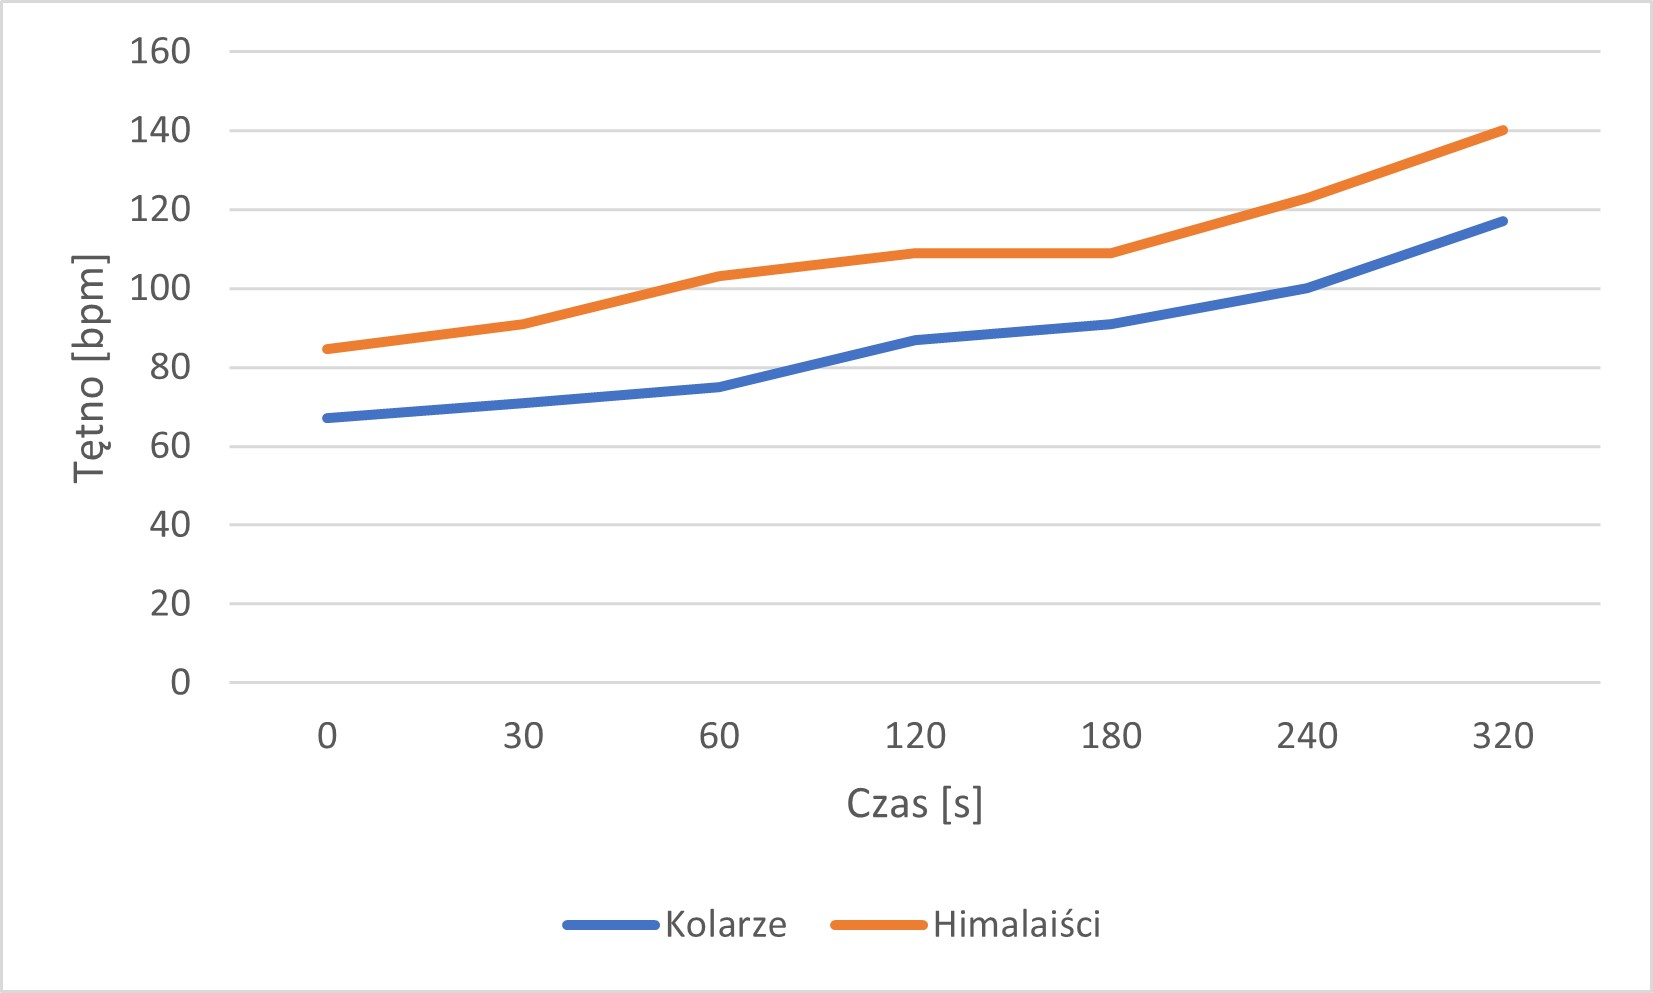
\includegraphics[width=.9\linewidth]{tetno.jpg}
    \caption{Porównanie zmiany czasowej średniej wartości tętna kolarzy oraz himalaistów podczas badania}
\end{figure}
\section{Analiza Wyników Himalaistów}
Wszyscy przebadani himalaiści dotrzymali do końca badania. Puls tych osób zaczął spadać dopiero w 240. sekundzie badania, a na końcu grupa ta osiągnęła najwyższy poziom saturacji. Największa różnica w czasie reakcji została odnotowana po rozpoczęciu badania, ale podobnie jak w pierwszej grupie, prawdopodobnie wynika to z zmiany pozycji na mniej znaną i komfortową. Wraz z upływem czasu badania czas reakcji stopniowo wzrastał. Tętno bardzo szybko wzrastało wśród prawie wszystkich himalaistów, czasami dochodząc do prawie dwukrotności początkowej wartości. Po wykonaniu badania osoby przebadane informowały, że najtrudniejszym okresem badania był czas między 180 a 240 sekundą, a w późniejszym okresie badania czuli się lepiej niż w tym czasie, co oznacza, że najlepiej dostosowali się do środowiska spośród wszystkich grup.
\begin{figure}[!htb]
    \centering
    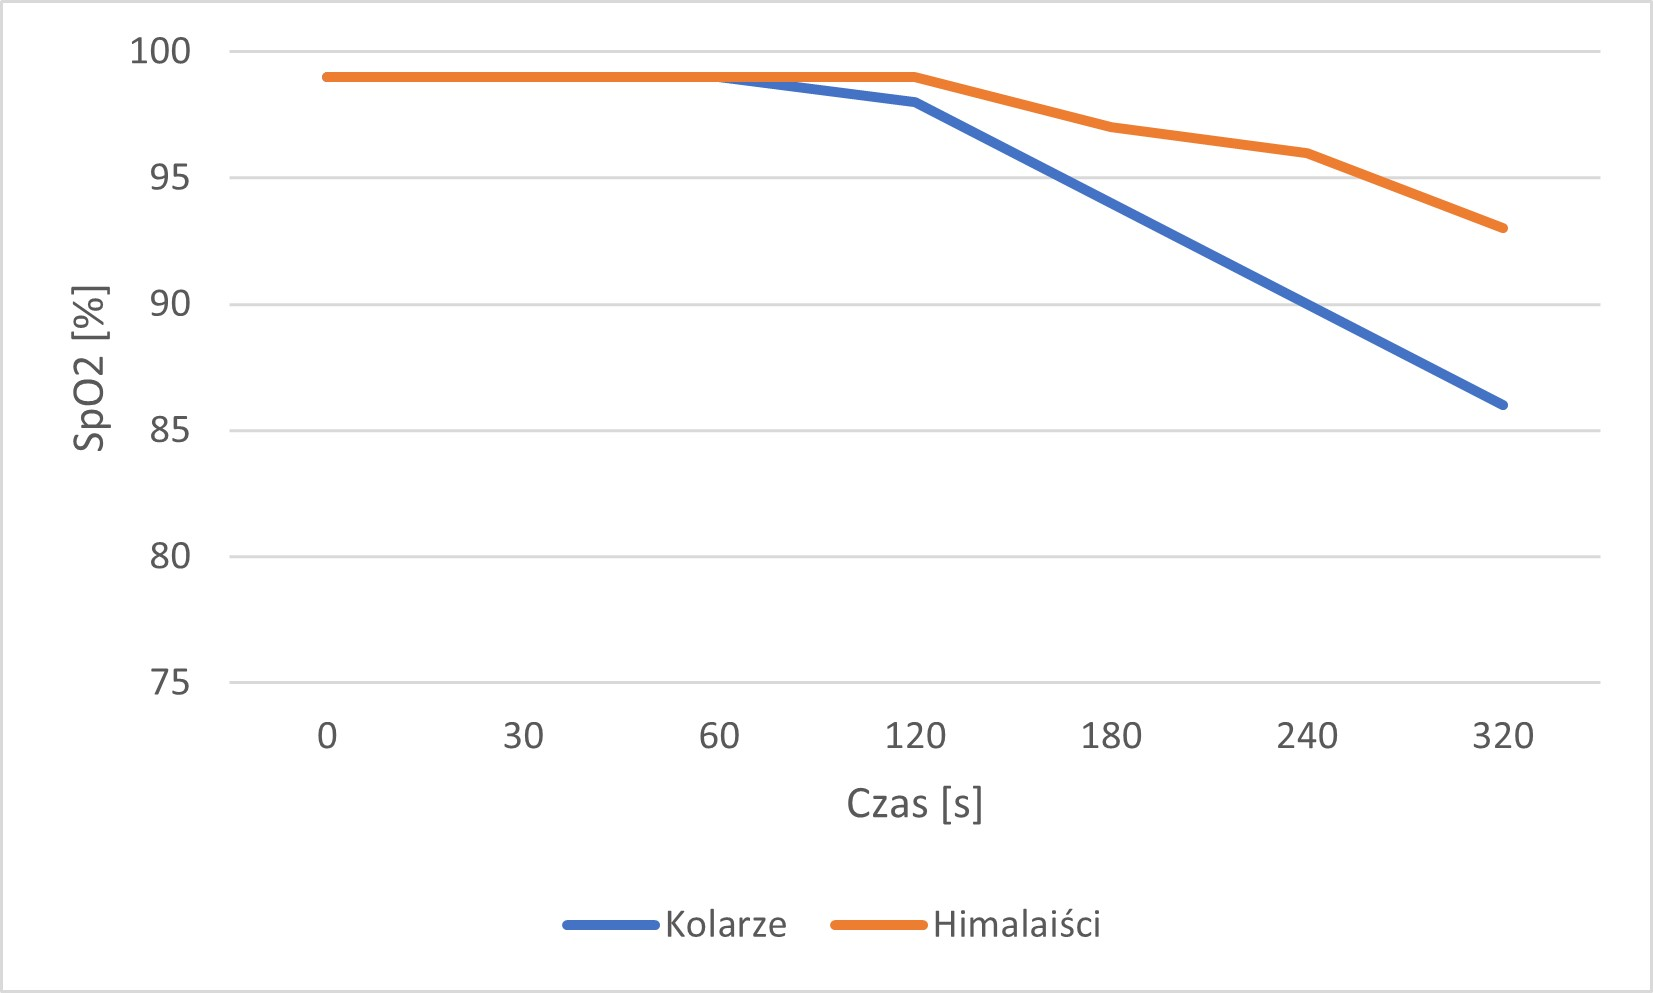
\includegraphics[width=.9\linewidth]{saturacja.jpg}
    \caption{Porównanie zmiany czasowej średniej wartości saturacji kolarzy oraz himalaistów podczas badania}
\end{figure}



\section{Analiza Całościowa}
Osoby nieaktywne fizycznie wykazały się największą podatnością na przygotowane środowisko, co może wynikać z mniejszej tolerancji na wysiłek. Kolarze, dzięki niskiemu tętnu i przygotowania do wykonywanego ćwiczenia, prezentowali bardziej efektywne dostosowanie do środowiska. Himalaiści osiągnęli najlepsze wyniki w saturacji krwi i utrzymywali stabilność czasu reakcji, co może sugerować ich wysoką adaptacyjność do warunków ekstremalnych.

W celu bardziej szczegółowego zrozumienia różnic między grupami himalaistów, a koalrzy w zakresie saturacji krwi, przeprowadzono test t-Studenta. Wynik testu wyniósł p = 0,004344. Uzyskana p-wartość jest poniżej standardowego poziomu istotności statystycznej 0,05. Oznacza to, że istnieją statystycznie istotne różnice w saturacji krwi między badanymi grupami. Odrzucenie hipotezy zerowej sugeruje, że różnice te nie są wynikiem przypadku, ale są bardziej związane z rzeczywistymi różnicami w badanych parametrach.